\documentclass[a4paper, 12pt]{article}
\usepackage{geometry}
\geometry{verbose,a4paper,tmargin=2cm,bmargin=2cm,lmargin=2cm,rmargin=2cm}
\usepackage[T2A]{fontenc}
\usepackage[utf8]{inputenc}
\usepackage[english,russian]{babel}
\usepackage{graphicx}

\newif\ifisinsp
\newif\ifisone
\newif\ifisname
\newif\ifisnum
\isinsptrue
\isonetrue
\isnamefalse
\isnumtrue

\def \labtype {Лабораторная}
% Это для нумерации страниц после титульника
\usepackage{fancyhdr}
\pagestyle{fancy}
\renewcommand{\headrulewidth}{0pt}
\fancyfoot[C] {\thepage}

\isonefalse
\def \labnum {3}
\def \labsubj {Системы ввода/вывода и периферийные устройства}
\def \labauthor {Мохнаткин Д.А. \\ Шумеев А.А.}
\def \labgroup {P3418}
\def \labinsp {Быковский С.В.}
\def \labname {Вариант 5}
\isnametrue

\begin{document}
\begin{titlepage}
	\begin{center}
		\large
		Университет ИТМО

		\vspace{0.25cm}
		
		Факультет программной инженерии и компьютерной техники
		
		Кафедра информатики и прикладной математики
		\vfill
		
		\textsc{\labtype\space работа \ifisnum № \labnum{} \fi по дисциплине \\"\labsubj" \ifisname\small \\ \labname \fi}
			
		\bigskip
	\end{center}
	\vfill
	\vfill
	
	\begin{flushright}
	\ifisone
	Выполнил: \labauthor
	\else
	Выполнили: \labauthor
	\fi

	\vspace{0.25cm}
	Группа: \labgroup
			
	\vspace{0.25cm}
	\ifisinsp
	Проверяющий: \labinsp
	\fi
	\end{flushright}
	\vfill
	
	\begin{center}
	СПб, \the\year
	\end{center}
\end{titlepage}

\tableofcontents

\newpage
\section{Задание}
Программное обеспечение soft-процессора Microblaze должно выполнять функции программного обеспечения из Лабораторной работы №1 и №2.
Программное обеспечение Microblaze должно определять период сигнала, поданного на вход capturetrig0 блока AXI Timer и выводить значение периода на дискретные порты ввода/вывода блока AXI GPIO.
Блок Output Compare должен быть настроен на генерацию сигнала outs с заданным периодом. Период передается по последовательному каналу и принимается с помощью блока AXI Uartlite.
В аппаратном обеспечении выход outs блока Output Compare подается на вход capturetrig0 блока AXI Timer.

\section{Структурная схема разработанной системы}
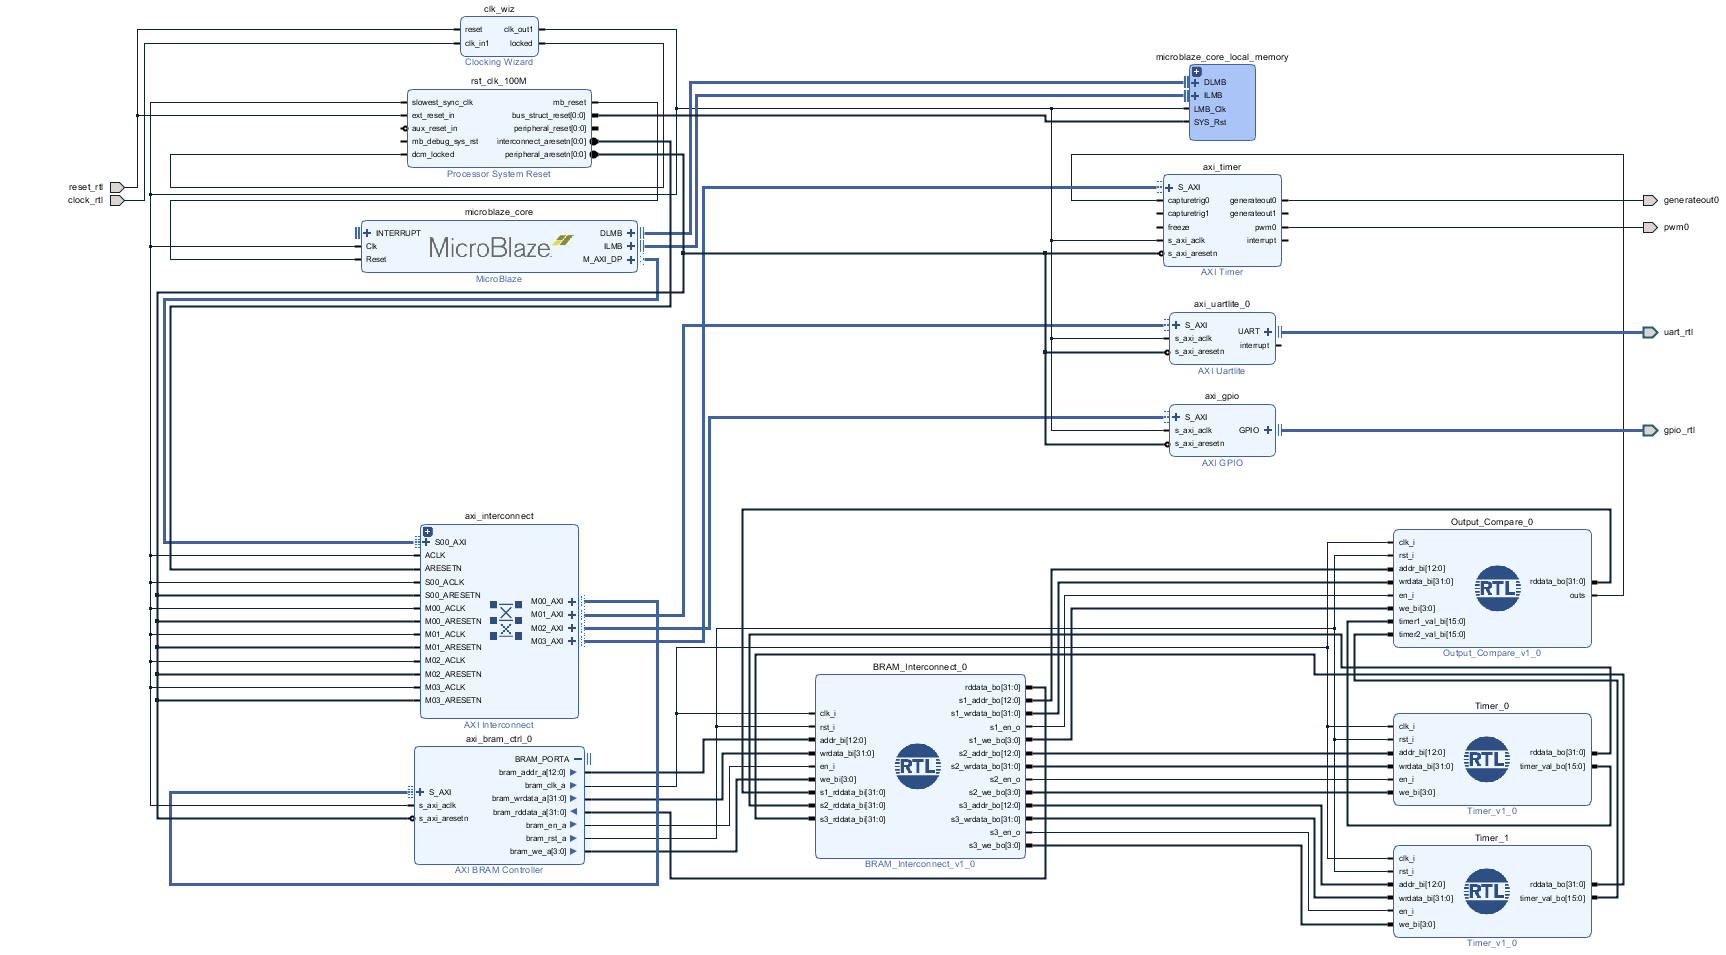
\includegraphics[width=\textwidth]{scheme.png}

\section{Блок-схема организации программного обеспечения процессора}
%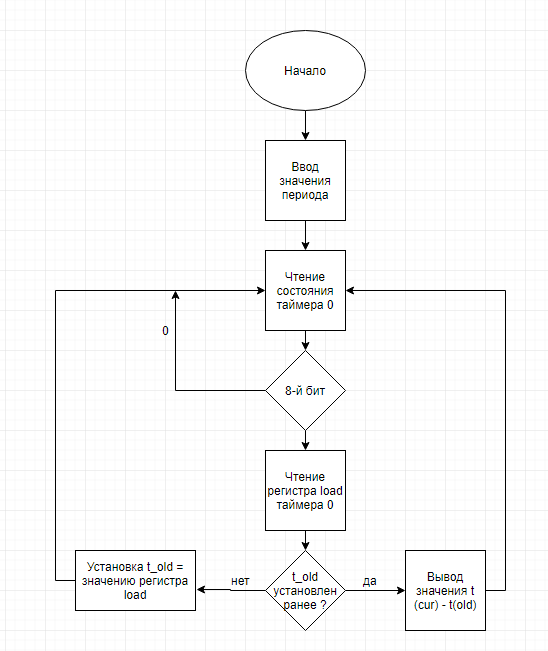
\includegraphics{io_lab2/block_scheme.png}

\section{Отчет о тестировании функциональности разработанной системы}
\subsection{Тест 1 ($t_{0}$ = $t_{1}$)}
%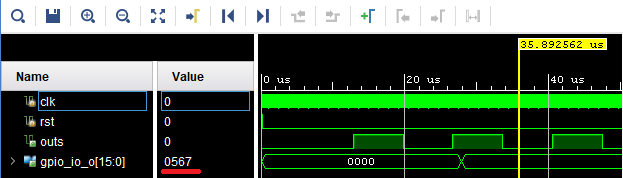
\includegraphics{io_lab2/test1.png}
\subsection{Тест 2 ($t_{0}$ $\neq$ $t_{1}$)}
%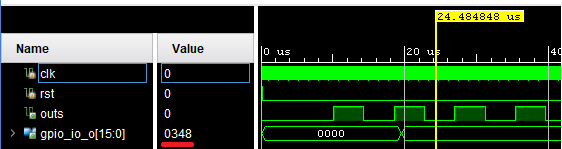
\includegraphics{io_lab2/test2.png}

\section{Известные ограничения}
\begin{enumerate}
	\item На вход принимаются 3-х значные числа в десятичной системе счисления.
	\item Введенное число не должно быть слишким маленьким ($\geq$300). Данное ограничение появляется из-за способа определения переполнения axi\_timer (реализовано через переодический опрос регистра состояния таймера). Ограничение может быть снято, если определять переполнение axi\_timer по прерыванию (требует изменение структурной схемы).
\end{enumerate}

\section{Выводы по работе}
\begin{enumerate}
\item Получены навыки разработки контроллеров ввода/вывода с использованием языка Verilog HDL для микропроцессорной системы с soft-процессором Microblaze.
\item В ходе работы ознакомились с процедурой прототипирования разработанной микропроцессорной системы на ПЛИС.
\end{enumerate}
\end{document}